\scanpage{88}
\mspage{1.}
% A reversed typescript is visible through the sheet.
$\unsure{\mathfrak X|\mathscr X|\mathcal X}$ schéma formel régulier, \inserted{connexe}, $\mathfrak X_0=X_0$ diviseur régulier, $D\deleted{\unsure{=}}=\bigcup_0^{\unsure{r|n}}D_i$ diviseur \deleted{avec} normal crossings \unsure{seulement|deux à deux} $D_0=X_0$, [les $D_i$ réguliers \unsure{individuellement|irréductibles}] . $D'=\sum_{i\ne0}D_i$, $D'_0$ induit sur $X_0$.

\figure{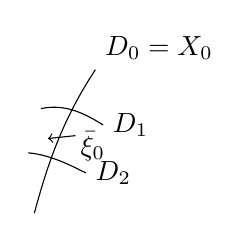
\begin{tikzpicture}[x=.52cm,y=.52cm]
\draw (-.65,-1.6) .. controls (-.3,-.3) and (.08,.75) .. (.84,1.9) node[above right] {$D_0=X_0$};
\draw (-.49,.95) .. controls (.11,1.08) and (.6,.82) .. (1.03,.55) node[right] {$D_1$};
\draw (-.8,-.13) .. controls (-.2,-.18) and (.37,-.51) .. (.61,-.62) node[right] {$D_2$};
\draw[->] (.35,.29)--(-.32,.22);
\node[right] at (.24,.03) {$\bar\xi_0$};
\end{tikzpicture}}

\diagram{\begin{tikzcd}[ampersand replacement=\&,column sep=.52em,row sep=.45em]
 e\arrow[r]\& I_0\arrow[r]\& \pi_1^t(\mathfrak X/D,\bar\xi_1)\arrow[r]\& \pi_1^t(X_0/D'_0,\bar\xi_0)\arrow[r]\&e\\
 {}\&{}\&\pi_1^t(\mathfrak X/D)\arrow[u,equal]\&\pi_1^t(U)\arrow[u,equal]\&\pi_1(\mathfrak X/D',\bar\xi_{\unsure{1|0}})\arrow[ul,equal]\\
 {}\&{}\&{}\&D_0-D'_0\arrow[u,equal]\&\Bigg\}
\end{tikzcd}}

\diagram{\begin{tikzcd}[ampersand replacement=\&,column sep=1.25em,row sep=.5em]
 \deleted{\unsure{\mu}}\arrow[r]\&\mu^\infty_{X_0,\mathrm{tame}}(\bar\xi_0)\arrow[r]\& I_0\arrow[r]\&0\\
 {}\&\mu(\deleted{\unsure{\bar\xi}})\arrow[u,equal]\&{}\&{}
\end{tikzcd}}
\margin{$=\varprojlim_{n>0}\mu_n$ \ $n$ inversible dans $\mathcal O_{X_0}$}

\diagram{\begin{tikzcd}[ampersand replacement=\&,column sep=1.2em,row sep=.3em]
 \mu\arrow[r]\& I\arrow[r]\&0\\
 \mu^\infty_{X_0,\mathrm{tame}}\arrow[u,equal]\&{}\&\text{faisceaux étale sur }X_0
\end{tikzcd}}

Donc
\[
 \prod_{\ell\,\unsure{\mathcal O_{X_0}=\mathcal O_{X_0}|\mathcal O_{X_0}^{*}|\ne p}}\mathbb Z_{\ell}
\]
\[
 \mu(\bar\xi_0)\longrightarrow\pi_1^t(\mathfrak X/D)\longrightarrow\pi_1^t(U)\longrightarrow e
\]

Opération de $\pi_1^t(U)$ sur $I_0$ via opérations de $\pi_1^{\unsure{t}}(U)$ sur $\deleted{\unsure{I}}\mu$ \deleted{\unsure{via opé|via opér.} ---}. Extension donnée par
\[
 \alpha\deleted{\unsure{\xi}}\in H^2(\pi_1^t(U),I_0)
 \qquad\qquad \deleted{\unsure{\xi}}\alpha=\,?
\]

% slanted
\margin{for all $H^i$, $i>0$, \uline{true} if $D_0$ \uline{is \uline{curve} over a} \uline{field}}
\uline{Lemme} 1. Soit $\widetilde U^t$ rev. étale de $U$ défini par $\pi_1^t$. Alors $H^1(\widetilde U^t,J\inserted{\text{constant}})=0$ si $\unsure{\#J|\mathcal J}$ premier aux car. résiduelles de $X_0$ [p. ex. $J=I$].

% slanted
\margin{Serre-Hochschild $H^{*}(U,J)\Leftarrow H^p(\pi_1^t,H^q(\widetilde U^t,\widetilde J))$}
\diagram{\begin{tikzcd}[ampersand replacement=\&,column sep=.55em,row sep=.35em]
0\arrow[r]\&H^2(\pi_1^t,I)\arrow[r,"\rho"]\& H^2(U,I)\arrow[r]\& H^2(\widetilde U^t,I_0\inserted{\text{constant sur }\widetilde U^t})^{\pi_1^t}\arrow[r]\& \bigl[H^3(\pi_1^t,I)\arrow[d]\\
{}\&{}\&{}\&\operatorname{Hom}(H_2(\widetilde U^t),I)^{\pi_1^t}\arrow[u,equal]\&\bigl.H^3(U,I)\bigr]\\
{}\&{}\&{}\&\operatorname{Hom}(\pi_2^t(U),I)^{\pi_1^t}\arrow[u,equal]\&{}
\end{tikzcd}}

\deleted{\unsure{f|$\rho$} \unsure{can.}} Donc $\alpha$ connu quand on connaît $\rho(\alpha)$, et l'image de \unsure{plus|$\rho(\alpha)$} dans $H^2(\widetilde U^t,I)^{\pi^t}\simeq\operatorname{Hom}(\pi_{2}^t(U),I)^{\pi_1^t}$ est nulle.
% archive sheet number: 87
